\documentclass[12pt,a4paper]{report}
\usepackage[utf8]{inputenc}
\usepackage[T1]{fontenc}
\usepackage{lmodern}
\usepackage{ngerman}
\usepackage{graphicx}
\usepackage{hyperref}
\bibliographystyle{plain}
\begin{document}
\begin{titlepage}
	\centering
	
\includegraphics[width=0.8\textwidth]{Hochschule_162}\par\vspace{1cm}
	\vspace{1cm}
	{\scshape\Large Bachelorarbeit\par}
	\vspace{1.5cm}
	{\huge\bfseries Bergepanzer M32 / M74\par}
	\vspace{2cm}
	{\small\bf vorgelegt von\par}
	{\Large\itshape Alexander Osiik und Alonso Essenwanger\par}
	\vfill
	betreut von\par
	Malte \textsc{Schmitz}

	\vfill

% Bottom of the page
	{\large L\"ubeck, den \today\par}
\end{titlepage}
\pagebreak

\tableofcontents 
\begin{abstract} 
In dieser Bachelorarbeit geht es um den Bergepanzer M32/M74. Diese basierten basierten auf dem Chassis des M4 Sherman und waren die ersten Bergepanzer der US Army mit Kranausstattung. 
\end{abstract} 
\newpage
\renewcommand\abstractname{Summary}   
\begin{abstract} 
This bachelor's thesis deals with the armoured recovery vehicle M32/M74. These were based on the chassis of the M4 Sherman and were the first armoured recovery vehicle of the US Army with crane equipment.  
\end{abstract} 
\chapter{Einleitung} 
\section{Was ist der Sinn dieses Projekts?} 
Es geht um das Erlernen des Umgangs mit \LaTeX. 
\subsection{Aufgabenstellung} 
Suchen Sie sich einen interessanten und nicht zu langen Wikipedia-Artikel und verwandeln Sie diesen in eine von Ihnen verfasste fiktive Bachelorarbeit. Setzen Sie diese Arbeit mit \LaTeX. 

\chapter{Bergepanzer M32}
\section{Entwicklung}
\par 
Als während des {\bf Zweiten Weltkrieges} dringlicher Bedarf für ein leistungsstarkes Fahrzeug zur Bergung ausgefallener oder abgeschossener Panzer erkennbar wurde, begann man beim {\bf US Ordnance Corps} mit der Entwicklung eines ausreichend dimensionierten Bergepanzers. Aus Zeitgründen benutzte man das Fahrgestell des in Großserie gebauten {\bf M4 Sherman} und rüstete dieses lediglich für die entsprechenden Bedürfnisse um. Das neue Fahrzeug erhielt die Bezeichnung {\it M32 Tank Recovery Vehicle}.
\par
Anstelle des Turms wurde ein fester Aufbau angebracht und ein "'A''-förmiger sechs Meter langer Kranbaum mit einer Hubleistung von 15 Tonnen installiert. Die Haupt-Bergewinde hatte eine maximale Zugkraft von 30 Tonnen. In der Panzerwanne wurde ein 81-mm-Mörser montiert, außerdem war das Fahrzeug noch mit einem {\bf 12,7-mm-Browning M2 Maschinengewehr} bewaffnet.


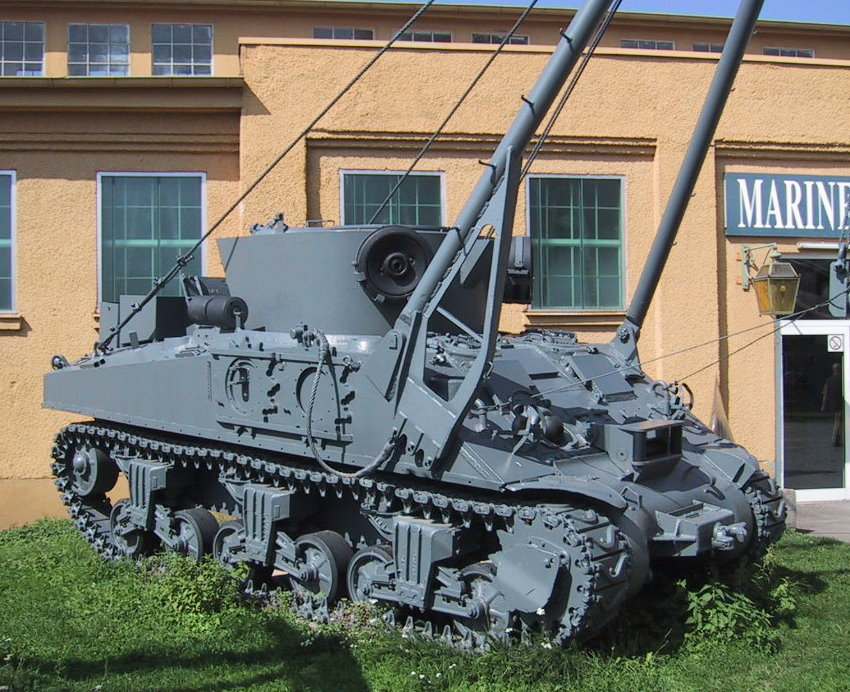
\includegraphics[trim = -19cm 0 0 -9cm,scale=0.2]{M32}
\\
\noindent\hspace*{25mm}$http://www.bbbahn.eu/M32_Speyer_30.8.08a1.jpg$

\pagebreak

\section{Varianten}
Es gab im Laufe der Zeit verschiedene Modelle des Bergepanzers M32.
\begin{itemize}
\item {\bf M32B1} – Umgerüstet aus dem M4A1. 24 Fahrzeuge wurden im März 1944 zu gepanzerten Artilleriezugmaschinen Prime Mover M34 umgebaut.
\item {\bf M32A1B1} – M32B1 mit HVSS-Laufwerk (horizontale Schraubenfederung und auf 58 cm verbreiterte Kette). Der Mörser wurde entfernt und die Krantechnik verbessert.
\item {\bf M32B2} – M32 Bergepanzer auf dem Fahrgestell des M4A2.
\item {\bf M32B3} – M32 Bergepanzer auf dem Fahrgestell des M4A3.
\item {\bf M32A1B3} – M32B3, auf den Standard des M32A1B1 modifiziert.
\item {\bf M32B4} – M32 Bergepanzer auf dem Fahrgestell des M4A4.
\end{itemize}

\chapter{Bergepanzer M74}
\section{Entwicklung}

\par
In Anbetracht der immer schwerer werdenden Kampfpanzer musste der M32 einer Leistungssteigerung unterzogen werden. Hierfür wurden Fahrgestelle des M4A3 HVSS verwendet und dem Fahrzeug die neue Bezeichnung M74 gegeben. Obwohl der M74 seinem Vorgänger ähnlich sah, gab es doch einige gravierende Unterschiede. Unter anderem wurde eine zweite Seilwinde für den Kranbaum eingebaut und am Bug befestigte man einen Stützschild für den Kranbetrieb, der bedingt auch als Räumschild einsetzbar war.
\par
Das Modell M74B1 entstand aus modifizierten M32B3. Die Bundeswehr nutzte dieses Fahrzeug als ihren ersten Bergepanzer. Von 1956 bis 1967 befanden sich 300 M74B1 im Einsatz.

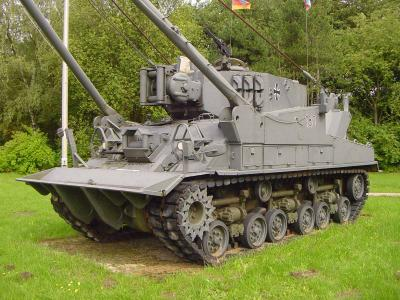
\includegraphics[trim = -9cm 0 0 -5cm,scale=0.4]{M74}
\\
$http://www.modellbau-magazin.de/fotos/12012404RS102410/12012404RS102410-100.jpg$

\chapter{Technische Daten}

\begin{tabular}{l|l}
	Gewicht:& 42,5 t Tonnen\\
	Motor:& Ford GAA, 8-Zylinder-Reihen-4-Takt-Vergasermotor, 506 PS\\
	Geschwindigkeit:& 34,5 km/h\\
	Besatzung:& 4 Mann\\
	Bugwinde:& 40 Tonnen maximale Zugkraft\\
	Krananlage (A-Mast):& 20 Tonnen maximale Hakenlast\\
	Zusätzlich:& Räumschaufel\\
\end{tabular}



\chapter{Hersteller}
\begin{itemize}
   \item {\bf Chrysler} im Detroit Tank Arsenal
   \item Fisher Body Division der {\bf General Motors Company} in Detroit (Michigan)
   \item {\bf Ford Motor Company} in Detroit (Michigan)
   \item Pacific Car and Foundry in South Renton (Washington)
   \item Federal Machine and Welder Company in Jersey City (New Jersey)
   \item Lima Locomotive Works in Lima (Ohio)
   \item Montreal Locomotive Works in Montreal (Québec)
\end{itemize}

\pagebreak

\begin{thebibliography}{999}
\bibitem [Marx] -Marx, Stefan: Die Bergepanzer der Bundeswehr und die deutsche Bergetechnik. Tankograd Militärfahrzeuge Spezial No. 5005, Tankograd Publishing, 2004.
\bibitem [PM] -Bergepanzer M-32: \url{http://www.panzer-modell.de/referenz/in_detail/m32/m32.htm} – [Online; Zugriff am 13.12.2016]
\bibitem [PM] -Bergepanzer M-74: \url{http://www.panzer-modell.de/berichte/m74_hp/m74.htm} – [Online; Zugriff am 13.12.2016]


\end{thebibliography}

\end{document}

